\documentclass{article}
\usepackage{graphicx}
\graphicspath{{./img/}}
\title{2411 HW 3}
\author{Duncan Wilkie}
\date{24 September 2021}

\begin{document}

\maketitle

\section*{1a}
The total error is the sum of the roundoff and approximaiton errors.
We can find critical points of this error function to determine its minimum in terms of $N$.
For the trapezoid rule, the total error
\[E=\frac{1}{N^2}+10^{-15}\sqrt{N}\]
is extremized when
\[\frac{dE}{dN} = 0\Leftrightarrow \frac{-2}{N^3}+\frac{10^{-15}}{2\sqrt{N}} = 0\Leftrightarrow N=(4\times 10^{15})^{2/5}=1.741\times10^6\]
For Simpson's rule, the total error
\[E=\frac{1}{N^4}+10^{-15}\sqrt{N}\]
is extremized when
\[\frac{dE}{dN}=0\Leftrightarrow \frac{-4}{N^5}+\frac{10^{-15}}{2\sqrt{N}} = 0 \Leftrightarrow N = (8\times 10^{15})^{2/9}=3420.\]
Clearly, this shows that Simpson's rule has minimum total error for fewer points.

\section*{1b}
We evaluate the error expressions at the extremal $N$ values found above.
For the trapezoid rule, the minimum error is $1.649\times 10^{-12}$, and for Simpson's rule, the minimum error is $6.579\times10^{-14}$.
The latter is good to the pentultimate digit of machine precision.

\section*{2}
The program appears in the Script Files section.

A plot of the potential, its numeric gradient, and the theoretical electric field appears below, indicating good agreement between numeric and exact computation.

\[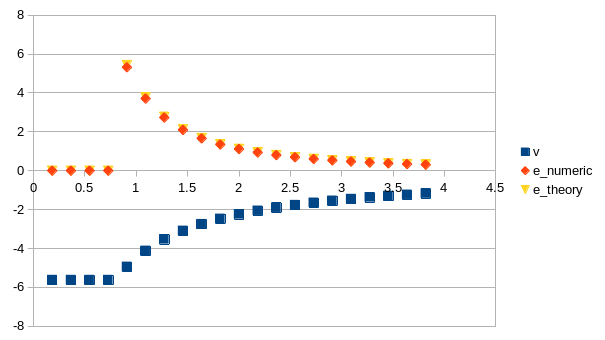
\includegraphics[scale=0.5]{plot1.png}\]

\section*{3}
The Taylor expansion of $f$ about $x_i$ is $f(x) = \sum_{n=0}^\infty\frac{f^{(n)}(x_i)}{n!}(x-x_i)^n$. The integral of this is $F(x) =\sum_{n=0}^\infty\frac{f^{(n)}(x_i)}{(n+1)!}(x-x_i)^{n+1}$. Since Simpson's rule truncates the expansions after $n=2$, $F(x)$ and the Simpson's rule integral agree to the $(x-x-i)^3$ term for each interval. Therefore, by the Lagrange form of the truncation remainder, the difference between them is bounded by the first neglected term of $F(x)$, i.e. $\frac{f^4(x_i)}{5!}(x-x_i)^5$, which is again bounded by $\frac{f^4(x_i)}{5!}h^5$ which is $O(2h^5/5!)f^4(x_i)$ as desired.

\section*{4}
The program appears in the Script Files section.

The plots of each method's absolute errors appear below, and indicate that extrapolated difference is the most accurate method for this problem. The extrapolated difference has what looks to be quartic error.

\[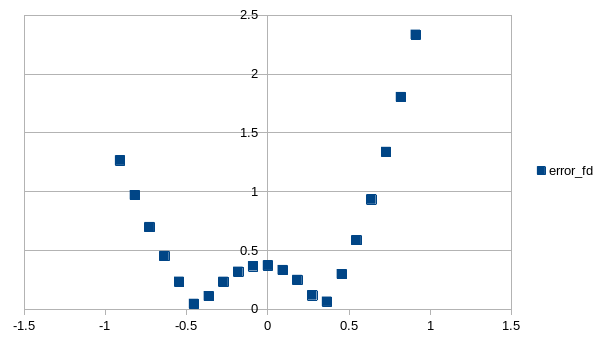
\includegraphics[scale=0.5]{plot2.png}\]
\[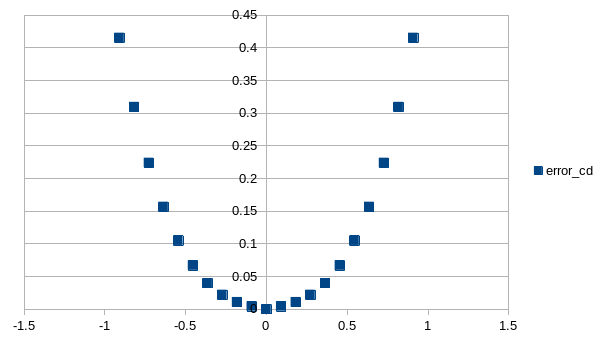
\includegraphics[scale=0.5]{plot3.png}\]
\[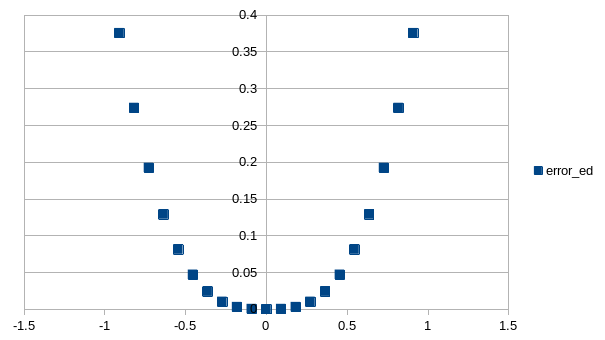
\includegraphics[scale=0.5]{plot4.png}\]

\section*{Script Files}
\subsection*{2}
\begin{verbatim}
Script started on Fri 24 Sep 2021 04:33:12 PM CDT
[dwilk14@tigers ~/HW3]$ cat dwilk14_hw3p2.cpp
#include <iostream>
#include <fstream>
#include <cmath>

using namespace std;

float V(float r) {
  if (r <= 0.80) {
    return -5.625;
  } else {
    return -4.5 / r;
  }
}

float E(float r) {
  if (r <= 0.80) {
    return 0.0;
  } else {
    return 4.5 / pow(r, 2);
  }
}

int main() {
  ofstream outfile;
  float a = 0.001, b = 4.0, h = 0.02, space = (b - a) / 22, x = a + space;
  outfile.open("output.txt");

  outfile << "x\tV\tNumerical E\tTheoretical E" << endl;

  for (int i = 0 ; i < 21; i++) {
    outfile << x << " " << V(x) << " " << (V(x + h) - V(x)) / h << " " << E(x) << endl;
    x += space;
  }

  return 0;

}
[dwilk14@tigers ~/HW3]$ g++ dwilk14_hw3p2.cpp -o dwilk14_hw3p2
[dwilk14@tigers ~/HW3]$ ./dwilk14_hw3p2
[dwilk14@tigers ~/HW3]$ cp dwilk14_hw3p2.txt /home3/kristina/phys2411/.
[dwilk14@tigers ~/HW3]$ exit
exit

Script done on Fri 24 Sep 2021 04:35:18 PM CDT

\end{verbatim}
\subsection*{4}
\begin{verbatim}
Script started on Fri 24 Sep 2021 04:35:36 PM CDT
[dwilk14@tigers ~/HW3]$ cat dwilk14_hw3p4.cpp
#include <iostream>
#include <fstream>
#include <cmath>

using namespace std;

double p4(double x) {
  return (3 - 30 * pow(x, 2) + 35 * pow(x, 4)) / 8;
}

double FD(double (*f)(double), double x, double h) {
  return (f(x + h) - f(x)) / h;
}

double CD(double (*f)(double), double x, double h) {
  return (f(x + h/2) - f(x-h/2)) / h;
}

double ED(double (*f)(double), double x, double h) {
  return 1 / (3 * h) * (8 * (f( x + h/4) - f(x - h/4)) - f(x + h/2) + f(x - h/2));
}

double exact(double x) {
  return 35 / 2 * pow(x, 3) - 7.5 * x;
}

int main() {
  ofstream outfile;
  outfile.open("output4.txt");
  double h = 0.1, a = -1, b = 1, step = (b - a) / 22, x = a + step;

  outfile << "x\tP_4(x)\tFD err\tCD err\tED err" << endl;

  for (int i = 0; i < 21; i++) {
    outfile << x << " " << p4(x) << " " << abs(FD(p4, x, h) - exact(x)) << " " \
        << abs(CD(p4, x, h) - exact(x)) << " " << abs(ED(p4, x, h) - exact(x)) << endl;

    x += step;
  }

  return 0;

}
[dwilk14@tigers ~/HW3]$ g++ dwilk14_hw3p4.cpp -o dwilk14_hw3p4
[dwilk14@tigers ~/HW3]$ ./dwilk14_hw3p4
[dwilk14@tigers ~/HW3]$ cp dwilk14_hw3p4.txt /home3/kristina/phys2411/.
[dwilk14@tigers ~/HW3]$ exit
exit

Script done on Fri 24 Sep 2021 04:36:39 PM CDT

\end{verbatim}

\end{document}
%%% Local Variables:
%%% mode: latex
%%% TeX-master: t
%%% End:
